%% LyX 1.3 created this file.  For more info, see http://www.lyx.org/.
%% Do not edit unless you really know what you are doing.
\documentclass[english, 12pt]{article}
\usepackage{times}
%\usepackage{algorithm2e}
\usepackage{url}
\usepackage{bbm}
\usepackage[T1]{fontenc}
\usepackage[latin1]{inputenc}
\usepackage{geometry}
\geometry{verbose,letterpaper,tmargin=2.5cm,bmargin=2.5cm,lmargin=2.5cm,rmargin=2.5cm}
\usepackage{rotating}
\usepackage{color}
\usepackage{graphicx}
\usepackage{subcaption}
\usepackage{amsmath, amsthm, amssymb}
\usepackage{setspace}
\usepackage{lineno}
\usepackage{hyperref}
\usepackage{bbm}


%\usepackage{xr}
%\externaldocument{SCT-supp}

\linenumbers
\doublespacing
%\usepackage[authoryear]{natbib}
\usepackage{natbib} \bibpunct{(}{)}{;}{author-year}{}{,}

%Pour les rajouts
\usepackage{color}
\definecolor{trustcolor}{rgb}{0,0,1}

\usepackage{dsfont}
\usepackage[warn]{textcomp}
\usepackage{adjustbox}
\usepackage{multirow}
\usepackage{graphicx}
\graphicspath{{../figures/}}
\DeclareMathOperator*{\argmin}{\arg\!\min}

\let\tabbeg\tabular
\let\tabend\endtabular
\renewenvironment{tabular}{\begin{adjustbox}{max width=0.9\textwidth}\tabbeg}{\tabend\end{adjustbox}}

\makeatletter

%%%%%%%%%%%%%%%%%%%%%%%%%%%%%% LyX specific LaTeX commands.
%% Bold symbol macro for standard LaTeX users
%\newcommand{\boldsymbol}[1]{\mbox{\boldmath $#1$}}

%% Because html converters don't know tabularnewline
\providecommand{\tabularnewline}{\\}

\usepackage{babel}
\makeatother


\begin{document}


\title{Making the most out of Clumping and Thresholding}
\author{Florian Priv\'e,$^{\text{1,}*}$ Bjarni J. Vilhj\'almsson,$^{\text{2}}$ Hugues Aschard$^{\text{3}}$ and Michael G.B. Blum$^{\text{1,}*}$}



\date{~ }
\maketitle

\noindent$^{\text{\sf 1}}$Laboratoire TIMC-IMAG, UMR 5525, Univ.\ Grenoble Alpes, CNRS, La Tronche, France, \\
\noindent$^{\text{\sf 2}}$National Center for Register-based Research, Aarhus University, Denmark. \\
\noindent$^{\text{\sf 3}}$Centre de Bioinformatique, Biostatistique et Biologie Int\'egrative (C3BI), Institut Pasteur, Paris, France,

\noindent$^\ast$To whom correspondence should be addressed.\\

\noindent Contacts:
\begin{itemize}
\item \url{florian.prive@univ-grenoble-alpes.fr}
\item \url{bjv@econ.au.dk}
\item \url{hugues.aschard@pasteur.fr}
\item \url{michael.blum@univ-grenoble-alpes.fr}
\end{itemize}

\newpage

\abstract{

}


%%%%%%%%%%%%%%%%%%%%%%%%%%%%%%%%%%%%%%%%%%%%%%%%%%%%%%%%%%%%%%%%%%%%%%%%%%%%%%%%

\newpage

\section{Introduction}

Clumping and Thresholding (C+T, also called P+T) is a simple technique for computing Polygenic Risk Scores (PRS) based on Genome-Wide Assocation Studies (GWAS) summary statistics, and has been used for more than ten years \cite[]{euesden2014prsice,purcell2009common}.
C+T consists in making a simple sum of allele counts (genotypes), weighted by effect sizes from GWAS summary-statistics, after having restricted the variants included in this sum. The first step consists in keeping only one representative variant by region of linkage disequilibrium (LD) by discarding variants that are too correlated with this particular one. The second step removes variants that are not significant enough, based on p-value from the GWAS summary statistics.
The first step is called ``clumping'' and the second step is called ``thresholding''.

When applying C+T, one has to choose at least 3 hyper-parameters: for clumping, the squared correlation threshold $r_{c}^2$ and the window size $w_c$ of clumping [RENAME??]; for thresholding, the p-value threshold $p_T$.
More often than otherwise, C+T users fix default values for clumping, such as $r_{c}^2$ of 0.1 (default of PRSice), 0.2  or 0.5 (default of PLINK), and $w_c$ of 250kb (default of PRSice and PLINK) or 500kb, and test values for $p_T$ ranging from $1$ to $10^{-8}$ at most \cite[]{wray2014research,euesden2014prsice,chang2015second}.
Moreover, one need to use imputed data to get the same variants between the GWAS and the data to compute the PRS on. 
A liberal inclusion of variants is often accepted, with the assumption that the more variants there are in the model, the better would be the prediction, whatever the imputation accuracy of these variants. 
Here, we consider this threshold on quality of imputation (often called the INFO score) as a fourth parameter of the C+T method.

Here, we show that these four hyper-parameters are really important, and that choosing those hyper-parameters well could substantially increase the predictive power of C+T over using current default parameters.
We implement an efficient way to compute scores for many different parameters in our R package bigsnpr \cite[]{prive2017efficient}. 
Moreover, instead of choosing the set of parameters that corresponds to the best prediction, we show that stacking all scores improves prediction beyond the best prediction of any of those scores \cite[]{breiman1996stacked}. 
We call this method SCT, which stands for Stacked Clumping and Thresholding.
Using the UK Biobank data \cite[]{bycroft2017genome} and external summary statistics for simulated and real data analyses, we show that testing a larger grid of parameters consistently improves predictions as compared to using some default parameters for C+T. We also show that SCT consistenly improves predictions over any single C+T prediction.

%%%%%%%%%%%%%%%%%%%%%%%%%%%%%%%%%%%%%%%%%%%%%%%%%%%%%%%%%%%%%%%%%%%%%%%%%%%%%%%%

\section{Material and Methods}

\subsection{Simulations}

We use variants from the UK Biobank imputed dataset that have a minor allele frequency larger than 1\% and an imputation INFO score larger than 0.3. There are almost 10M such variants, we randomly choose 1M of them.
We restrict individuals to the ones referred as of White British ancestry by the UK Biobank and exclude all second individuals in each pair reported as related individuals by the UK Biobank \cite[]{bycroft2017genome}.
335,609 individuals remain and we split them in three sets: one for training (e.g.\ choosing the hyper-parameters) and one for testing (evaluating the models) for which we sample 10,000 different individuals in both sets; and one for computing summary statistics (GWAS) with the 315,609 remaining individuals.

For simulating phenotypes and computing summary statistics, we transform the data into hard calls by randomly sampling hard calls according to imputation probabilities.
For the train and test sets, we use data in dosage format.
This enables us to simulate phenotypes using the ``real'' underlying genotypes as hard calls and use the INFO score (imputation accuracies) reported for the UK Biobank data for the imputed data. [END CLEAR ENOUGH??]

We simulate binary phenotypes with a heritability $h^2 = 0.5$ using a Liability Threshold Model (LTM) with a prevalence of 10\% \cite[]{falconer1965inheritance}. We vary the number of causal variants (100, 10K, or 1M) in order to match a range of genetic architectures from low to high polygenicity.
Liability scores are computed from a model with additive effects only: we compute the liability score of the i-th individual as \(y_i = \sum_{j\in S_\text{causal}} w_j \widetilde{G_{i,j}} + \epsilon_i,\) where $S_\text{causal}$ is the set of causal SNPs, $w_j$ are weights generated from a Gaussian distribution $N(0, h^2 / \vert S_\text{causal} \vert)$, $G_{i,j}$ is the allele count of individual $i$ for SNP $j$, $\widetilde{G_{i,j}}$ corresponds to its standardized version (zero mean and unit variance for all SNPs), and $\epsilon$ follows a Gaussian distribution $N(0, 1 - h^2)$.

To compute summary statistics, we use Cochran-Armitage additive test \cite[]{zheng2012analysis}. Given that we restricted the data to have minimal population structure, this test based on contingency tables is much faster than using a logistic regression with 10 principal components as covariates (40 minutes vs 16 hours) while providing similar effect sizes and Z-scores (Figure \ref{fig:GWAS}).

Each simulation is repeated 10 times.

\subsection{Real summary statistics}

We also investigate prediction using real summary statistics from published GWAS, summarized in table \ref{tab:sumstats} \cite[]{buniello2018nhgri}.
[DATA??]

\begin{table}[h]
\caption{Available cases and controls in UK Biobank (UKBB) for many binary traits, along with corresponding published GWAS summary statistics (from GWAS that do not include UKBB).\label{tab:sumstats}}
\vspace*{0.5em}
\centering
\begin{tabular}{|l|c|c|c|c|c|}
  \hline
Trait & UKBB size & GWAS size & GWAS \#SNPs & GWAS citation \\
  \hline
Breast cancer (BRCA) & ~~10,690 / 159,163 & 137,045 / 119,078 & 11,792,542 & \cite{michailidou2017association} \\
Rheumatoid arthritis (RA) &  & ~~29,880 / ~~73,758 & ~~9,739,303 & \cite{okada2014genetics} \\
Type 1 diabetes (T1D) & ~~~~~~~768 / 314,570 & ~~~~~5913 / ~~~~~8828  & ~~8,996,866 & \cite{censin2017childhood} \\
Type 2 diabetes (T2D) & ~~14,156 / 314,570 & ~~26,676 / 132,532 & 12,056,346 & \cite{scott2017expanded} \\
Prostate cancer (PRCA) & ~~~~~6330 / 141,591 & ~~79,148 / ~~61,106 & 20,370,946 & \cite{schumacher2018association} \\
Depression (MDD) & ~~26,121 / 291,735 &   & 13,554,550 & \\
Coronary artery disease (CAD) & ~~12,263 / 225,927 & ~~60,801 / 123,504 & ~~9,455,778 & \cite{nikpay2015comprehensive} \\
Asthma & ~~43,787 / 261,985 & ~~19,954 / 107,715 & ~~2,001,280 & \cite{demenais2018multiancestry} \\
Celiac disease?? \\
   \hline
\end{tabular}
\end{table}

\subsection{Clumping and Thresholding (C+T) and Stacked C+T (SCT)}

We compute C+T scores for each chromosome separately and for many parameters:
\begin{itemize}
\item Threshold on imputation INFO score within \{0.3, 0.6, 0.9, 0.95\}.
\item Squared correlation threshold of clumping $r_{c}^2$ within \{0.01, 0.05, 0.1, 0.2, 0.5, 0.8, 0.95\}.
\item Base size of clumping window within \{50, 100, 200, 500\}. $w_c$ is then computed as the base size divided by $r_{c}^2$. For example, for $r_{c}^2 = 0.2$, we test values of $w_c$ within \{250, 500, 1000, 2500\} (in kb). This is motivated by the fact that linkage disequilibrium is inversely proportional to genetic distance between variants \cite[]{pritchard2001linkage}.
\item A sequence of 50 thresholds on p-values between 0.1 (-log10(p) = 1) and the most significant p-value, equaly spaced on a log-log scale.
\end{itemize}
Overall, we compute $22 \times 4 \times 7 \times 4 \times 50 = 123200$ vectors of polygenic scores.
Computation time is largely driven by the computation of clumping sets, which consists mainly in computing squared correlations between pairs of variants. So, to speed-up the overall computation, we cache the computation of those correlations.

Then, we stack all these polygenic scores (for individuals in the training set) by using these scores as variables in an efficient penalized logistic regression available in our R package bigstatsr \cite[]{prive2019efficient}.
This results in a linear combination of C+T scores from which we derive a single vector of  effect sizes. The resulting single vector of new effect sizes is used for evaluation in the test set. 
We refer to this method as SCT in the rest of the paper.

From this grid, we derive two scores: one using default parameters, i.e.\ with $r_{c}^2$ = 0.2, $w_c$ = 500, a liberal threshold of 0.3 on imputation INFO score, and choosing the p-value threshold ($\leq 10^{-8}$) maximizing the AUC on the training set; one corresponding to the set of the previous four parameters that maximizes AUC on the training set. 
We refer to these scores as ``std\_CT'' and ``max\_CT'' in the rest of the paper.
Note that, as opposed to SCT, C+T scores use the same set of parameters for all chromosomes.

%%%%%%%%%%%%%%%%%%%%%%%%%%%%%%%%%%%%%%%%%%%%%%%%%%%%%%%%%%%%%%%%%%%%%%%%%%%%%%%%

\section{Results}

\subsection{Simulations}


\subsection{Real summary statistics}

In table \ref{tab:AUC}, we report AUC values on the test set (mean and 95\% CI from 10,000 bootstrap samples) and the number of variants used in the final model.

\begin{table}[h]
\caption{AUC values on the test set of UKBB (mean [95\% CI] from 10,000 bootstrap samples) and the number of variants used in the final model.\label{tab:AUC}}
\vspace*{0.5em}
\centering
\begin{tabular}{|l|c|c|c|c|}
  \hline
Trait & std\_CT & max\_CT & SCT \\
  \hline
Breast cancer (BRCA) &  \\
Rheumatoid arthritis (RA) & \\
Type 1 diabetes (T1D) & 73.7 [69.4-77.8] & 76.6 [72.6-80.5] & 79.4 [75.5-83.2] \\
 & 13,169 & 156 & 160,756 \\
Type 2 diabetes (T2D) & \\
Prostate cancer (PRCA) & 64.9 [63.2-66.5] & 65.2 [63.6-66.8] & 67.2 [65.7-68.7] \\
 & 1683 & 610 & 461,733 \\
Depression (MDD) & 55.3 [54.5-56.1] & 60.0 [59.2-60.7] & 60.6 [59.8-61.3] \\
 & 202,175 & 155,037 & 504,886 \\
Coronary artery disease (CAD) & 59.9 [58.6-61.2] & 61.1 [59.9-62.4] & 64.0 [62.7-65.2] \\
 & 1184 & 87,572 & 315,373 \\
   \hline
\end{tabular}
\end{table}

[TALK ABOUT PARAMETERS FOR 10 BEST PREDICTIONS??]

Effects resulting from SCT have mostly the same sign as initial effects from GWAS, with some effects being largely unchanged, and others having an effect that is shrunk to 0 or completely 0, i.e.\ variants not included in the final model (Figure \ref{fig:eff-BRCA}).
[TALK ABOUT PARTICULAR CASES]



\begin{figure}[htb]
\centerline{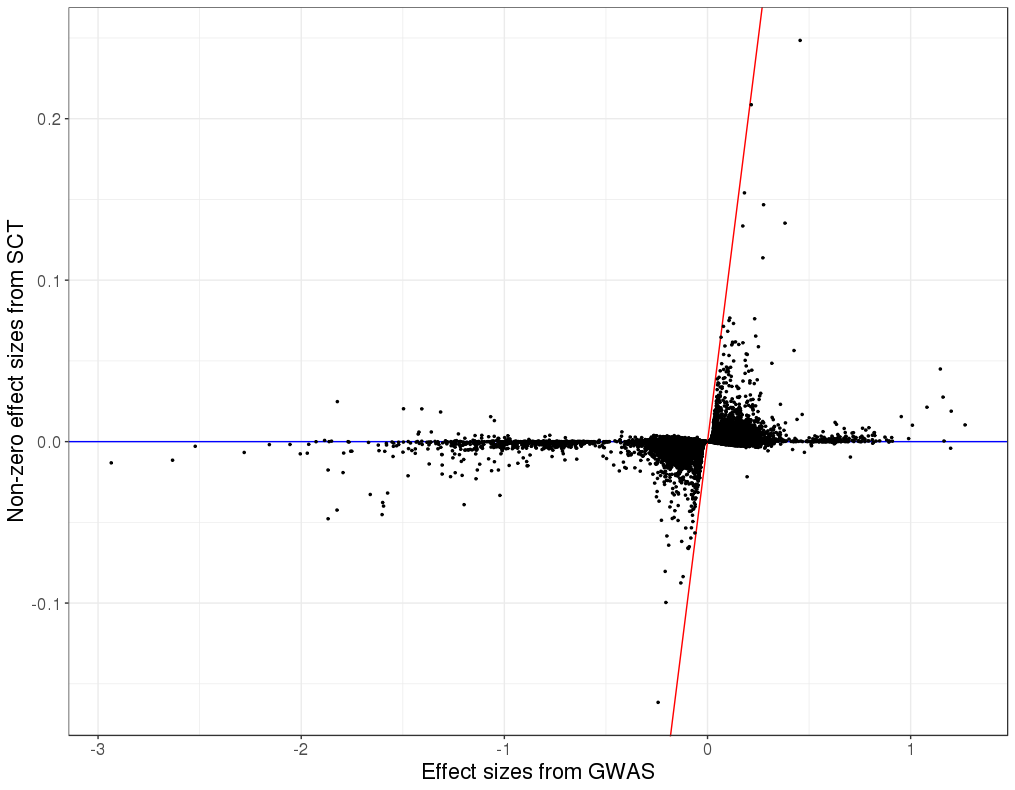
\includegraphics[width=0.7\textwidth]{new-effects-BRCA.png}}
\caption{Breast cancer. New effect sizes resulting from SCT versus initial effect sizes of GWAS. Only non-zero effects are represented. Red line corresponds to the 1:1 line.}
\label{fig:eff-BRCA}
\end{figure}

%%%%%%%%%%%%%%%%%%%%%%%%%%%%%%%%%%%%%%%%%%%%%%%%%%%%%%%%%%%%%%%%%%%%%%%%%%%%%%%%

\section{Discussion}




%%%%%%%%%%%%%%%%%%%%%%%%%%%%%%%%%%%%%%%%%%%%%%%%%%%%%%%%%%%%%%%%%%%%%%%%%%%%%%%%

\newpage

\section*{Acknowledgements}

Authors acknowledge LabEx PERSYVAL-Lab (ANR-11-LABX-0025-01) and ANR project FROGH (ANR-16-CE12-0033). Authors also acknowledge the Grenoble Alpes Data Institute that is supported by the French National Research Agency under the ``Investissements d'avenir'' program (ANR-15-IDEX-02).
This research has been conducted using the UK Biobank Resource under Application Number 25589.

%%%%%%%%%%%%%%%%%%%%%%%%%%%%%%%%%%%%%%%%%%%%%%%%%%%%%%%%%%%%%%%%%%%%%%%%%%%%%%%%

\newpage

\bibliographystyle{natbib}
\bibliography{refs}

%%%%%%%%%%%%%%%%%%%%%%%%%%%%%%%%%%%%%%%%%%%%%%%%%%%%%%%%%%%%%%%%%%%%%%%%%%%%%%%%

\newpage
\section*{Supplementary Data}

\renewcommand{\thefigure}{S\arabic{figure}}
\setcounter{figure}{0}
\renewcommand{\thetable}{S\arabic{table}}
\setcounter{table}{0}

\begin{figure}[htb]
\centerline{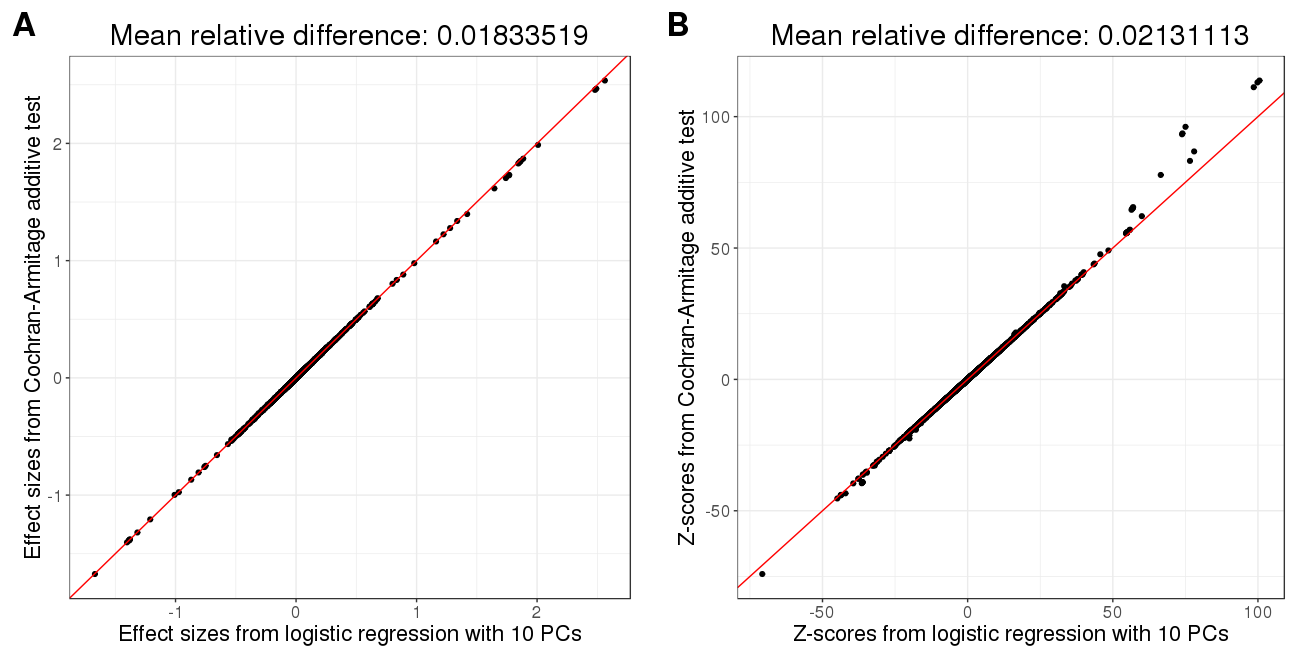
\includegraphics[width=0.95\textwidth]{equivalence.png}}
\caption{Comparison of estimated effect sizes (\textbf{A}) and Z-scores (\textbf{B}) if computed using a logistic regression with 10 principal components as covariates, or with a simple Cochran-Armitage additive test. Phenotypes were simulated using 100 causal SNPs only, allowing for large effects.}
\label{fig:GWAS}
\end{figure}

%%%%%%%%%%%%%%%%%%%%%%%%%%%%%%%%%%%%%%%%%%%%%%%%%%%%%%%%%%%%%%%%%%%%%%%%%%%%%%%%

\begin{figure}[htb]
\centering
\begin{subfigure}[b]{0.7\textwidth}
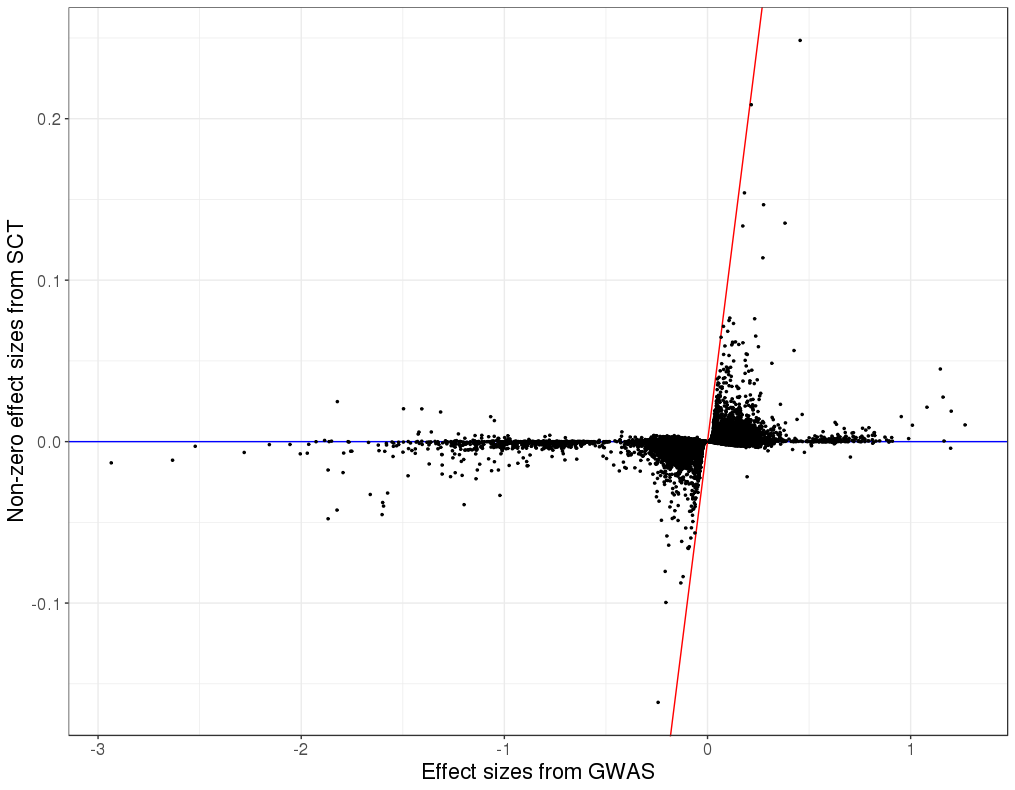
\includegraphics[width=\textwidth]{new-effects-BRCA.png}
\caption{Breast cancer}
\end{subfigure}
\\~\\~\\
\begin{subfigure}[b]{0.7\textwidth}
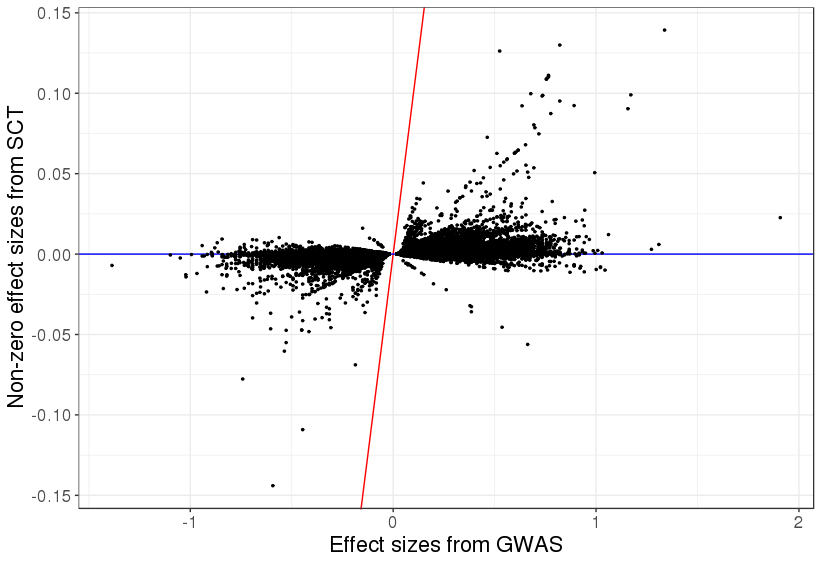
\includegraphics[width=\textwidth]{new-effects-RA.png}
\caption{Rheumatoid arthritis}
\end{subfigure}
\end{figure}

\begin{figure}[htb]\ContinuedFloat
\centering
\begin{subfigure}[b]{0.7\textwidth}
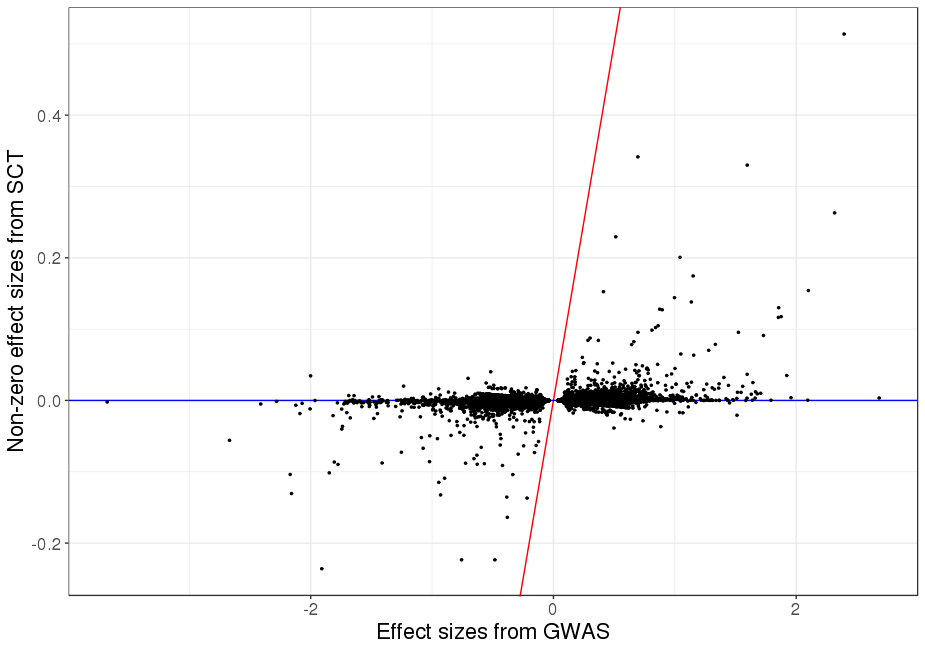
\includegraphics[width=\textwidth]{new-effects-T1D.png}
\caption{Type 1 diabetes}
\end{subfigure}
\\~\\~\\
\begin{subfigure}[b]{0.7\textwidth}
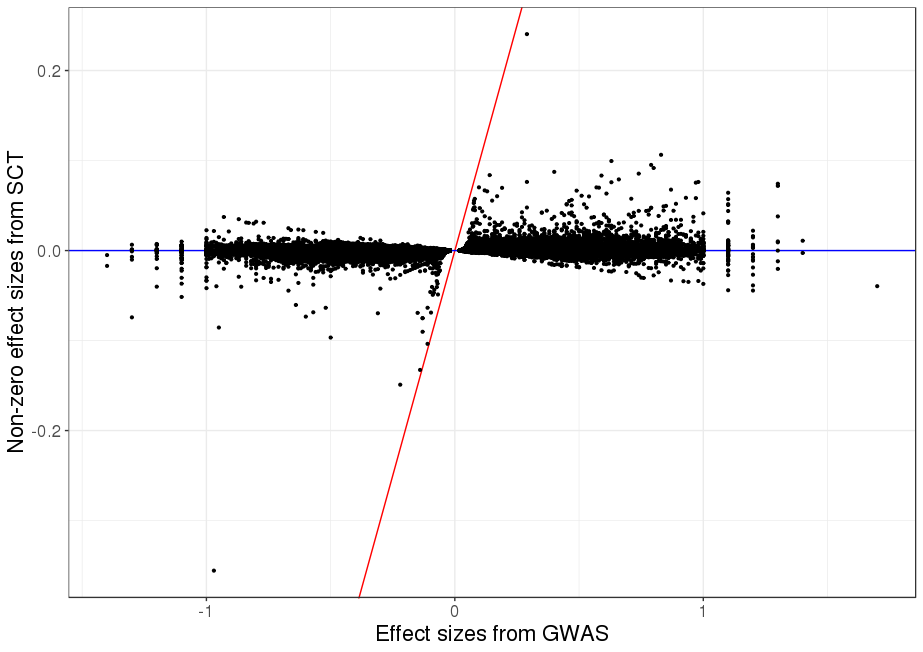
\includegraphics[width=\textwidth]{new-effects-T2D.png}
\caption{Type 2 diabetes}
\end{subfigure}
\end{figure}

\begin{figure}[htb]\ContinuedFloat
\centering
\begin{subfigure}[b]{0.7\textwidth}
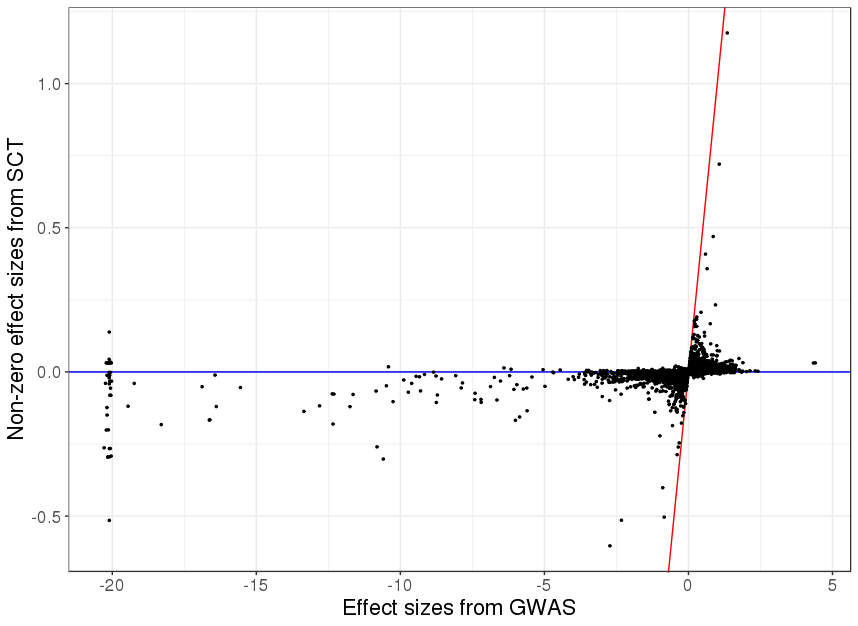
\includegraphics[width=\textwidth]{new-effects-PRCA.png}
\caption{Prostate cancer}
\end{subfigure}
\\~\\~\\
\begin{subfigure}[b]{0.7\textwidth}
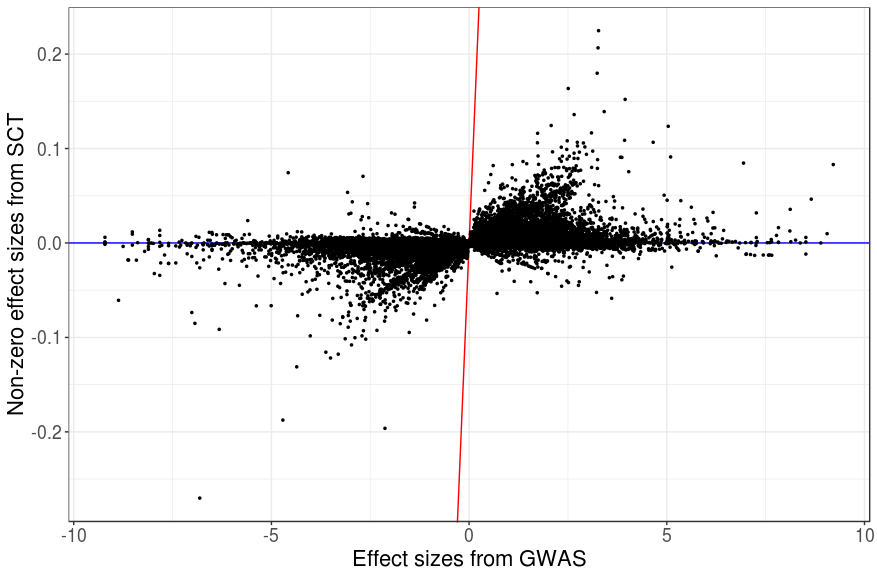
\includegraphics[width=\textwidth]{new-effects-MDD.png}
\caption{Depression}
\end{subfigure}
\end{figure}

\begin{figure}[htb]\ContinuedFloat
\centering
\begin{subfigure}[b]{0.7\textwidth}
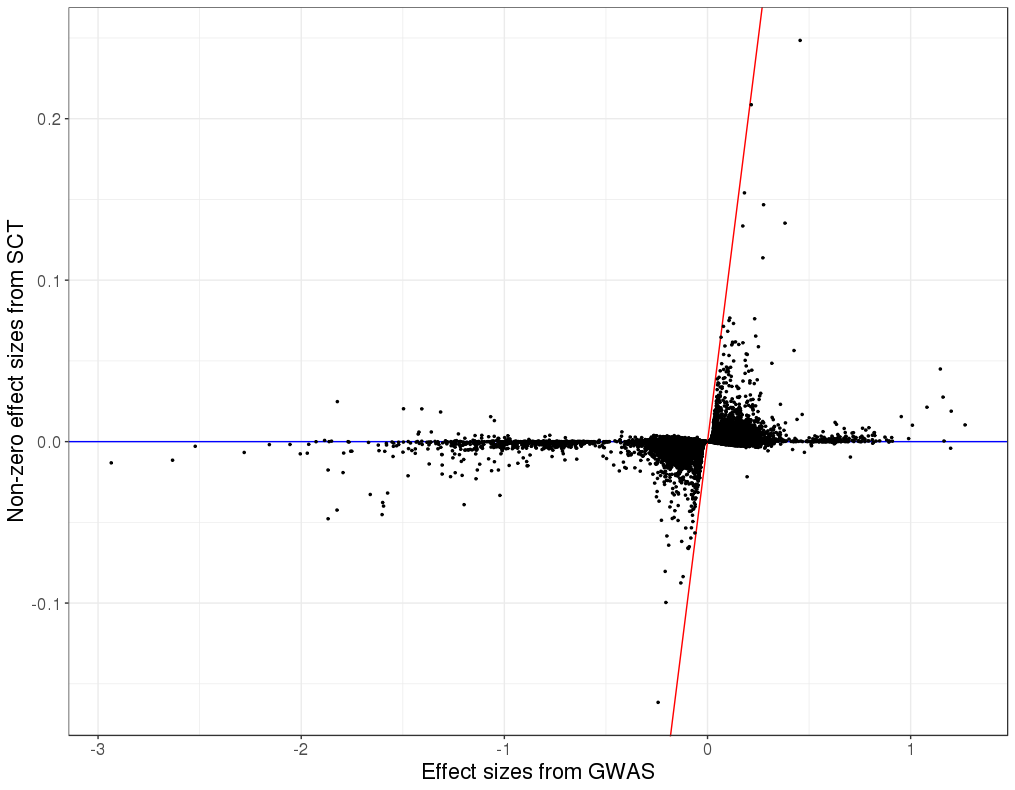
\includegraphics[width=\textwidth]{new-effects-BRCA.png}
\caption{Breast cancer.}
\end{subfigure}
\\~\\~\\
\begin{subfigure}[b]{0.7\textwidth}
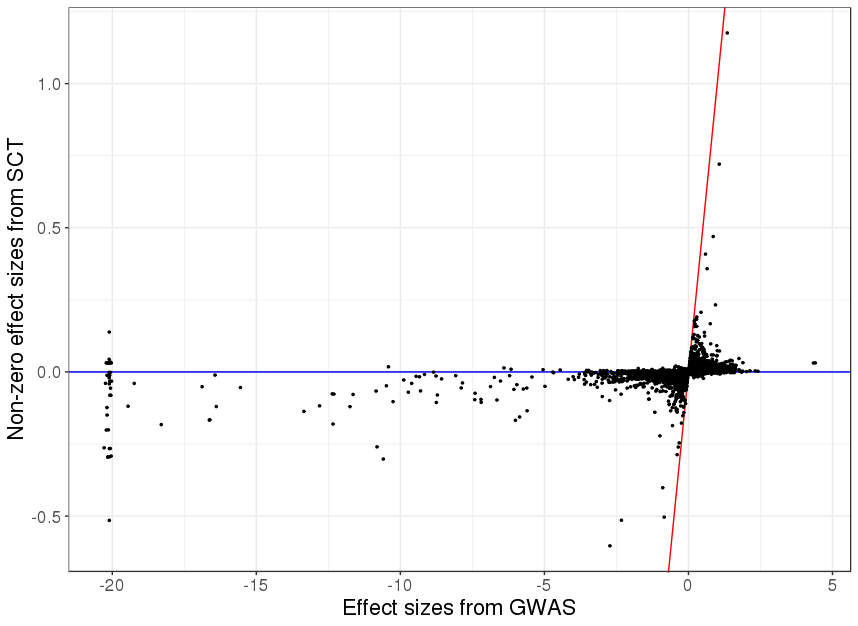
\includegraphics[width=\textwidth]{new-effects-PRCA.png}
\caption{Prostate cancer.}
\end{subfigure}
\caption{New effect sizes resulting from SCT versus initial effect sizes of GWAS. Only non-zero effects are represented. Red line corresponds to the 1:1 line.}
\end{figure}

%%%%%%%%%%%%%%%%%%%%%%%%%%%%%%%%%%%%%%%%%%%%%%%%%%%%%%%%%%%%%%%%%%%%%%%%%%%%%%%%

\begin{figure}[htb]
\centering
\begin{subfigure}[b]{\textwidth}
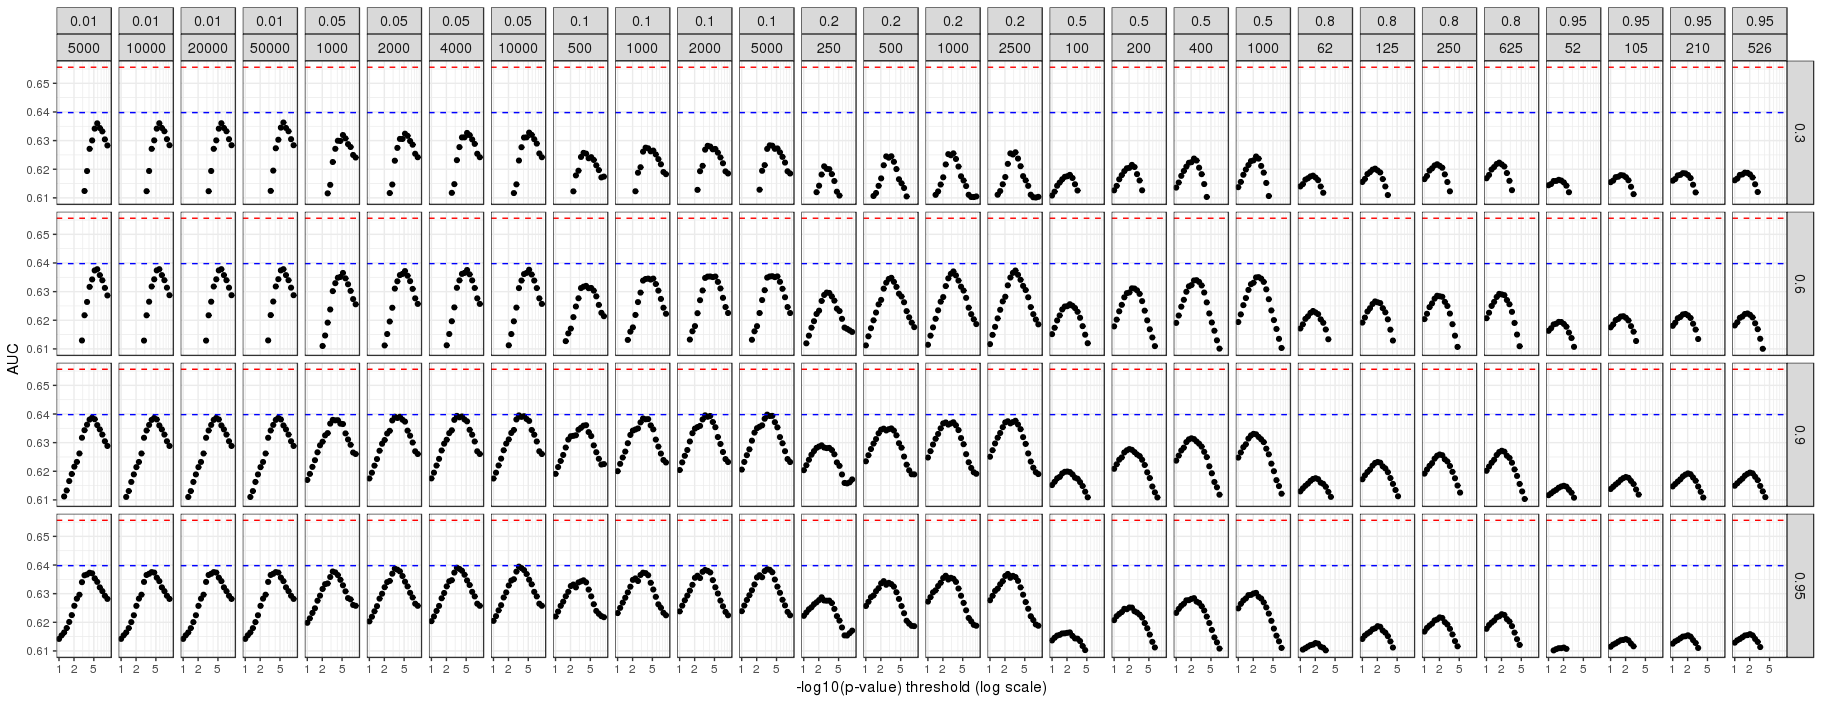
\includegraphics[width=\textwidth]{grid-BRCA.png}
\caption{Breast cancer}
\end{subfigure}
\\~\\
\begin{subfigure}[b]{\textwidth}
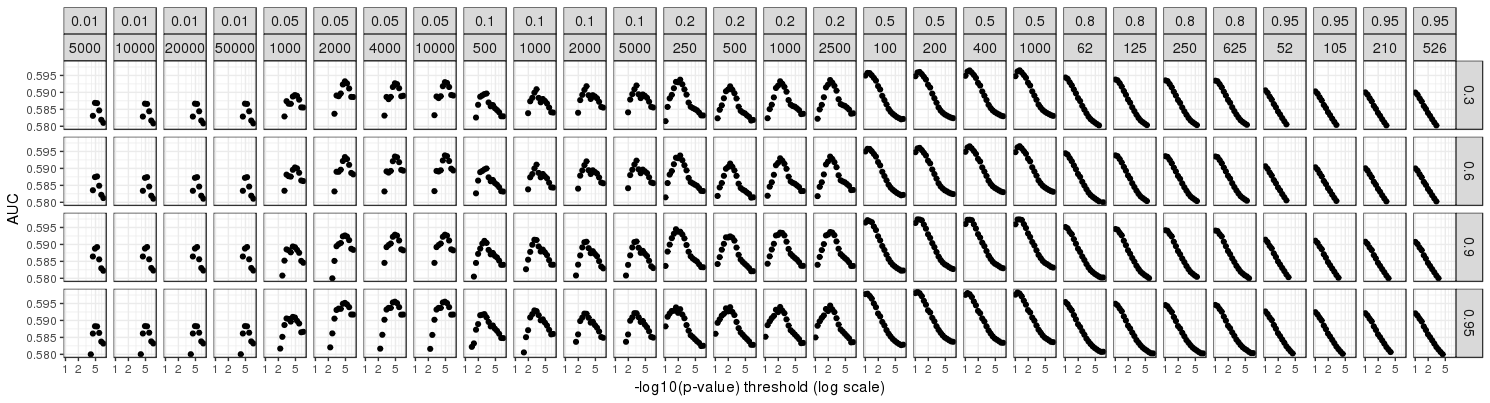
\includegraphics[width=\textwidth]{grid-RA.png}
\caption{Rheumatoid arthritis}
\end{subfigure}
\\~\\
\begin{subfigure}[b]{\textwidth}
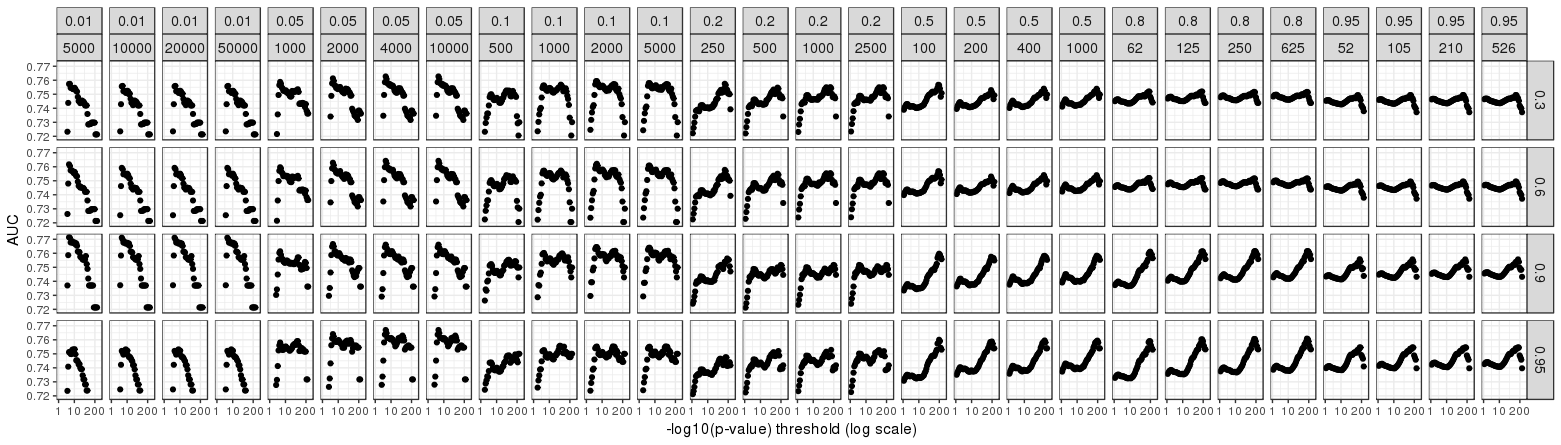
\includegraphics[width=\textwidth]{grid-T1D.png}
\caption{Type 1 diabetes}
\end{subfigure}
\end{figure}

\begin{figure}[htb]\ContinuedFloat
\centering
\begin{subfigure}[b]{\textwidth}
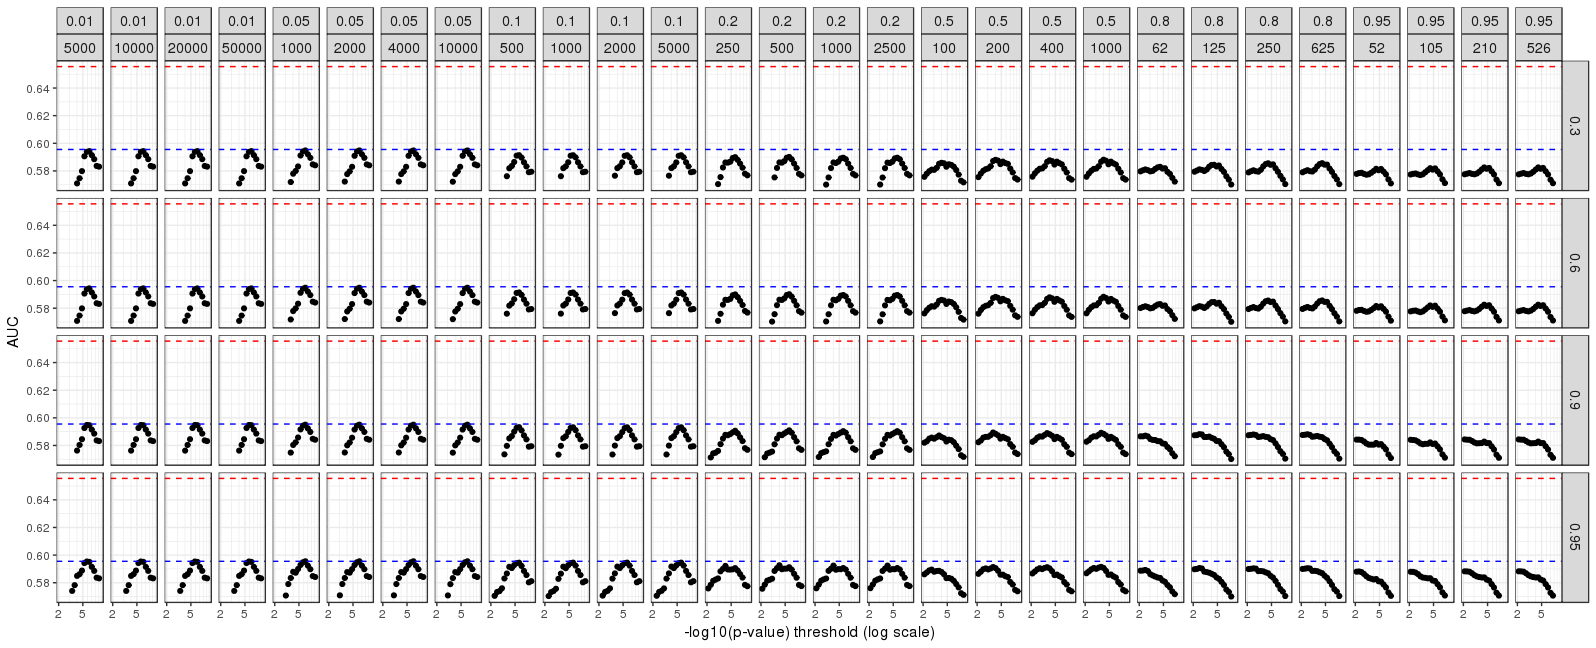
\includegraphics[width=\textwidth]{grid-T2D.png}
\caption{Type 2 diabetes}
\end{subfigure}
\\~\\
\begin{subfigure}[b]{\textwidth}
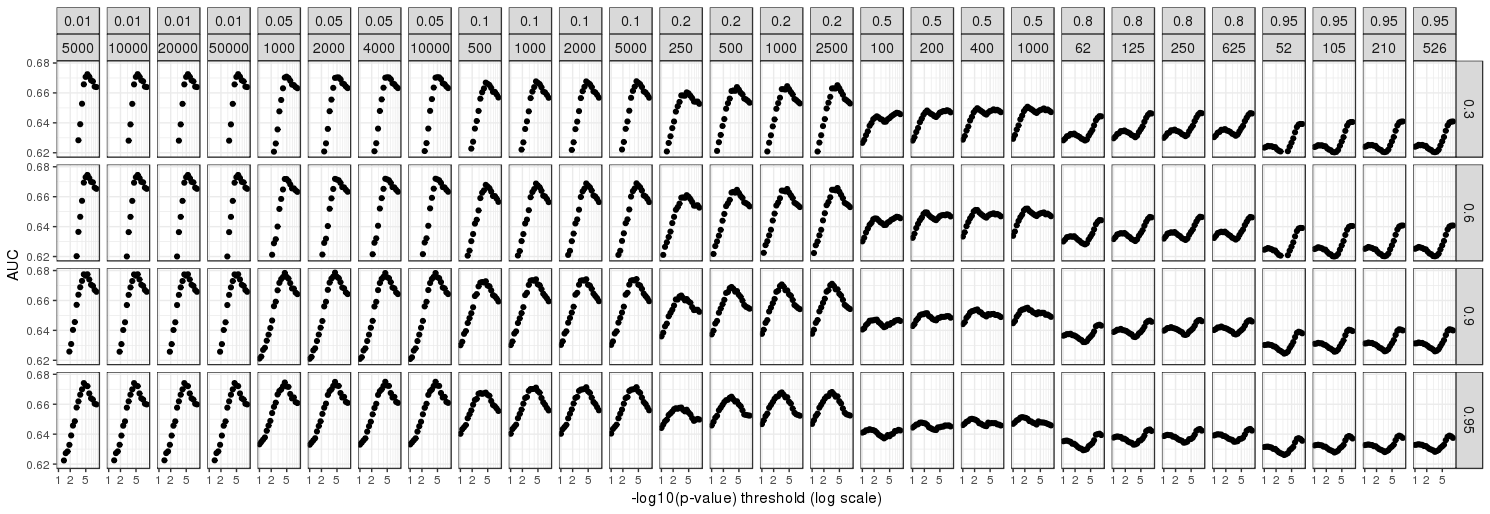
\includegraphics[width=\textwidth]{grid-PRCA.png}
\caption{Prostate cancer}
\end{subfigure}
\\~\\
\begin{subfigure}[b]{\textwidth}
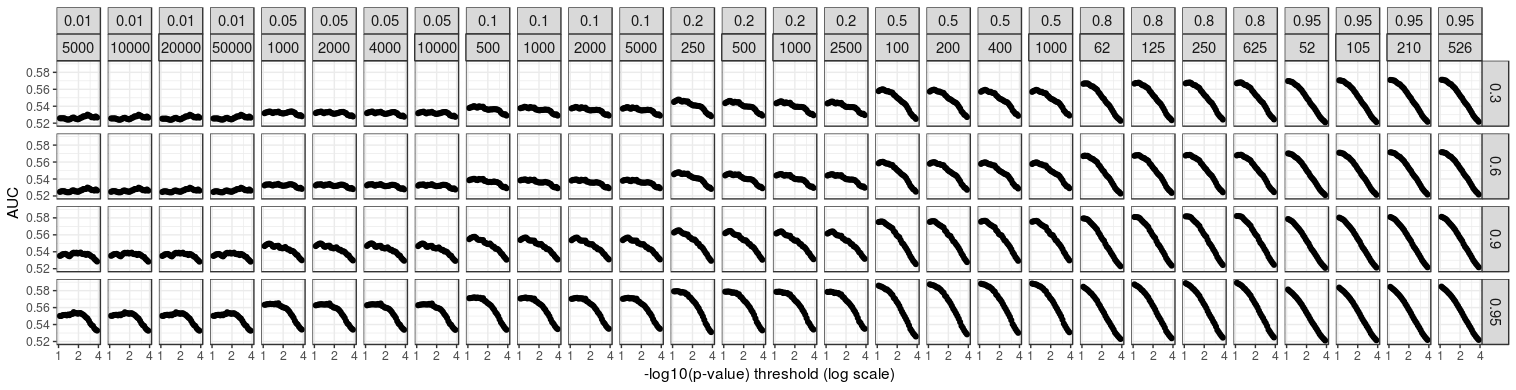
\includegraphics[width=\textwidth]{grid-MDD.png}
\caption{Depression}
\end{subfigure}
\end{figure}

\begin{figure}[htb]\ContinuedFloat
\centering
\begin{subfigure}[b]{\textwidth}
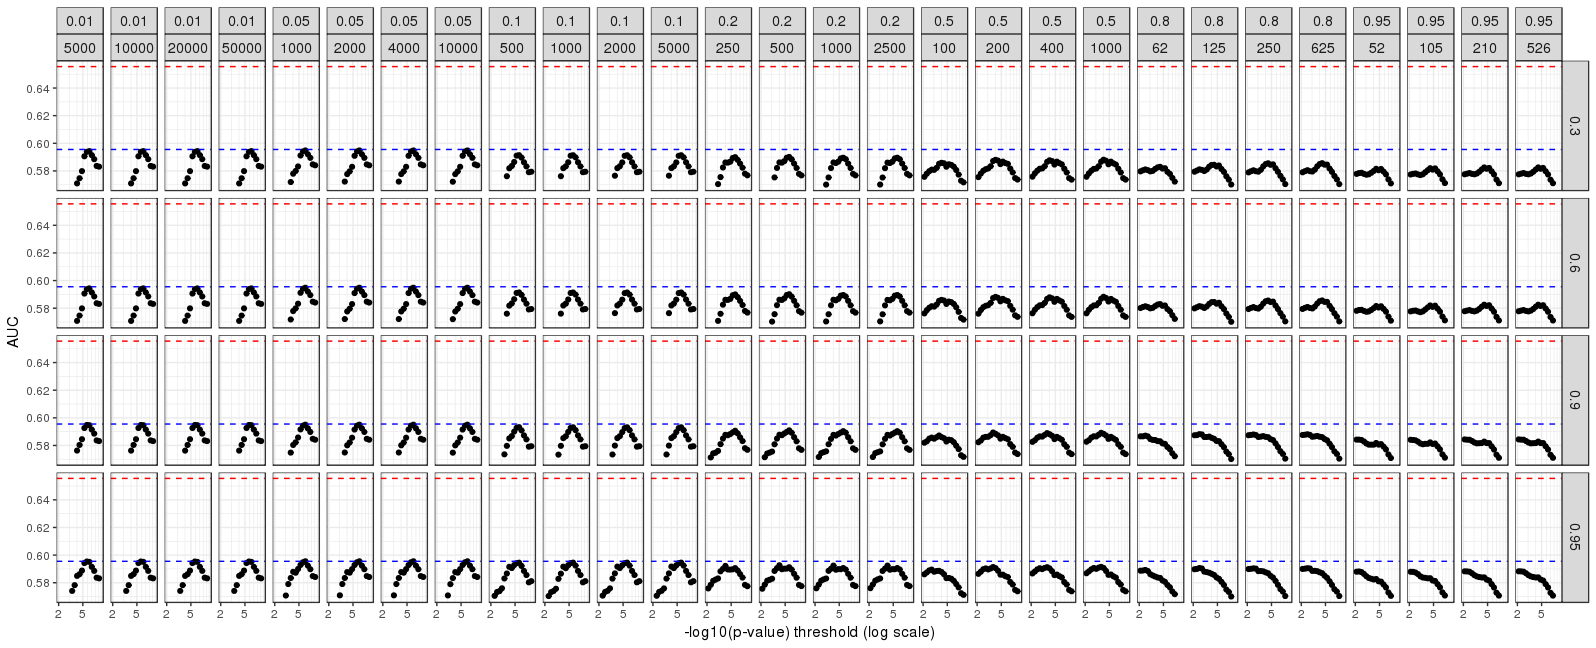
\includegraphics[width=\textwidth]{grid-T2D.png}
\caption{Type 2 diabetes}
\end{subfigure}
\\~\\
\begin{subfigure}[b]{\textwidth}
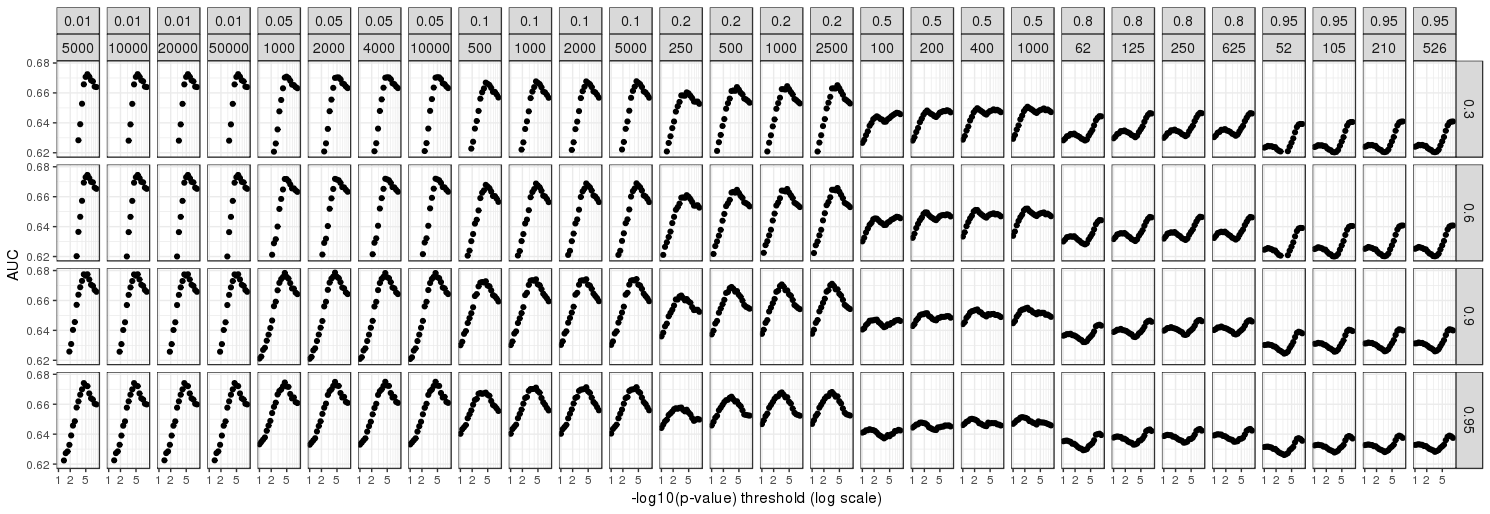
\includegraphics[width=\textwidth]{grid-PRCA.png}
\caption{Prostate cancer}
\end{subfigure}

\caption{AUC values when predicting disease status for many parameters of C+T. Blue line corresponds to the maximum AUC on the training set. Red line corresponds to AUC obtained with SCT on the test set. Facets are presenting different clumping thresholds $r_{c}^2$ from 0.01 to 0.95, window sizes $w_c$ from 52 to 50,000 kb, and imputation thresholds from 0.3 to 0.95. The x-axis corresponds to the remaining hyper-parameter, the p-value threshold $p_T$; here, -log10(p-values) are represented using a logarithmic scale.}
\end{figure}

\end{document}
